\documentclass[twoside]{report}

\usepackage{project}

\begin{document}

\begin{titlepage}
  %\vspace{12cm}
	\raggedright
  {\Large{\colorbox{front}{\color{white} \textbf{NORRSKEN}\kern 1pc}}\\\vspace{0.3cm}}
  {\texttt{Pilot Study}\\}
  \vfill
	{\large \today\par}
  {\small\color{gray} Marc Coquand, Linus Lagerhjelm, Mattias Cederberg and Simon
  Asp\\}
  {\small\color{gray} Supervised by Stig Byström}\\
  {\small\color{gray} Umeå University\\}

	%\vfill

\end{titlepage}

\newpage
\pagecolor{front}\afterpage{\nopagecolor}\thispagestyle{empty}

\marginpar{\textcolor{white}{\small{\texttt{Project
Management}}\vspace{11cm}\\\large\textbf{Summary}\\ {\small 
Walking home late at night can be a daunting experience. The newspapers write
about assaults and harassment, the northern winter climate contribute with
shorter days and darker nights. Existing street lights helps with the problem
but the feeling of uncertainty and fear persist. Norrsken will investigate
how a technical solution could be applied to create an increased sense of
safety. The project is carried out in collaboration with the municipality of
Umeå and Umeå University as part of the courses Interactivity in Smart
Environments and Project Management.
}}} 
 \newpage

\tableofcontents
\thispagestyle{empty}
\newpage

\section{Project Description}
\subsection{Purpose}
Design a proposal for a safe smart city environment where individuals’ personal
preferences and needs are met, build a demonstrator and, maybe, translate the
solutions to rural areas.
\subsection{Background}
Walking home late at night can be a daunting experience. The newspapers write
about assaults and harassment, the northern winter climate contribute with
shorter days and darker nights. Existing street lights helps with the problem
but the feeling of uncertainty and fear persist.
\subsection{Goals}
How can these smart environments (stretching over Ålidhem), and these
individuals’ activities be enriched with interactive, intelligent technology
for increasing safety?

Some interesting questions to solve also as part of this problem is: How can we
increase safety? How can we prototype a smart environment? What possibilities
are there to make the campus and surrounding environment smart? 

\subsection{Delimitations}
Our focus is only on the university area of Umeå. We will also limit us to only making a proof of concept.

\newpage

\section{Solution Proposal}
\marginfig{graphics/brainstorm.jpg}{Brainstorming session}
Our way to deal with the problem of safety is to create a more interesting city
which will generate more people moving around, which increases the feeling of
safety. We don’t want to arm the people of the city with tools to increase self
defense, rather creating a long term solution where the environment offers
safety. 

The solution we have come up with is to create a smart lighting system and a
display where you can get information about what’s going on on the campus area.
The place where this would be installed is at the new bicycle road that the
municipality will build. 

The lighting system will be an addition to the lights that are already there,
and the way we will get more people to move around is to enable interaction
between the people and the lights, so that something happens when they are
moving around. We also want to increase the brightness of the lights when there
is few people on the road so that they can see what’s going on the sides of the
road. 

The interactive display will be put out close to the road, or somewhere where
many people move around, for instance at a bus stop. The display will show what
is happening around campus and will be live updated so you easily can see which
lectures is held, which student pubs that are open et cetera. 

\newpage
\marginfig{graphics/intressent-analys.pdf}{The stakeholder analysis}
\section{Stakeholder Analysis}
\begin{rightsiderules}
As shown in the image, our core stakeholders is the supply
group. They are the ones that has the main interest in completing the project
and also has the most influence over the project. Our primary stakeholders is
the same as the projects clients, i.e. the municipality of Umeå.
Lastly, the secondary stakeholders. Those who will be affected by the project
somehow but will not take part in any decision making within the project.
\end{rightsiderules}

\section{Requirement Specification}

\subsection{Introduction}

Walking home late at night can be a daunting experience. The newspapers write
about assaults and harassment, the northern winter climate contribute with
shorter days and darker nights. Existing street lights helps with the problem
but the feeling of uncertainty and fear persist. This project will investigate
how a technical solution could be applied to increase safety. It is carried out
in collaboration with the municipality of Umeå and Umeå University as part of
the courses Interactivity in Smart Environments and Project Management.

Smart environments’ purpose is to either improve abilities, control something
or reduce/minimise unwanted events. It can therefore be interesting to see if
the technology can be applied to the problem of security in urban environments. 

In particular smart city technology, wearable computing or sensor networks can
perhaps be used to solve the problem of security. 

\subsection{Aim and Research Questions}

How can these smart environments (stretching over Ålidhem), and these
individuals’ activities be enriched with interactive, intelligent technology
for increasing safety? 

Some interesting questions to solve also as part of this
problem is: How can we increase safety? How can we prototype a smart
environment? What possibilities are there to make the campus and surrounding
environment smart? 

\subsection{Methods}

We initially conducted a user survey on what the user’s wanted to feel more
secure as well as figuring out what makes them feel insecure. From the results
two ideas were designed that will be presented to the Municipality. Depending on
the feedback that is received from the municipality one of the two ideas will be
continued and further developed. Mattias and the occupational therapists will be
responsible for the design while Marc, Simon and Linus will be responsible for
the technical implementation and prototypes. The goal is to develop a testable
prototype as early as possible so that it can be evaluated by the design group
with the help of users. This process is then repeated until we have a working
prototype that fulfills the requirements and goals of the project. 

\subsubsection{Use Scenarios}

Two people move to live in different apartments in the new campus area, and a
friend of theirs moves into an apartment at Ålidhem, nearby. They have different
routines, and different preferences regarding how and when conducting studies
and leisure activities. They have also different views on and strategies for
maintaining safety. Some are opposite strategies, such as avoiding crowds of
potentially threatening people, or seeing crowds as protection against
potentially hostile individuals.

\subsubsection{Anticipated Design Solution that will be Demonstrated January 10-11}

The demonstration will consist of a prototype and a proof of concept. It will then be presented with a live performance.  

\subsubsection{Requirements}
\begin{figure}[H]
\caption{The Functional Specification}
\begin{tabular}{|p{2.5cm}|l|l|l|l|}
  \hline
  & Requirement & Significance & Type of Requirement & Level of Significance
  \\\hline
  Complete in the end of January & O & R & F - Functional & M - Main function
  \\\hline
  Increase safety & D & M & D - Design Requirement & D - Desired
  \\\hline
  UI Prototype & F & R & P - Performance &
  \\\hline
  Concept art & F & R &  & 
  \\\hline
  Scenario Descriptions & F & R &  &
  \\\hline
  Anonymous & D & D & &
  \\\hline
  Proactive & D & R & &
  \\\hline
\end{tabular}
\end{figure}

\subsubsection{Material}

\begin{itemize}
    \item Wooden surfaces 
    \item Large paper (A3, A2)
    \item Motion sensor 
    \item A wifi-enabled microcontroller 
    \item Microphones.
    \item Projector
\end{itemize}

\subsection{Time Plan}

The project needs to be completed for a seminar the 11 of December. There will
also be a presentation the 15 of December as well as a presentation the 10 of
January. 

In December we expect to require access to sensor equipment and arduinos. We
might also need wooden surfaces and larger paper (A3, A2) for prototypes in
November and December. Alternatively we’ll need access to a projector or a big
screen (already done since the project has access to HUMlab). 

In particular some sort of sensors where the type is depending on what project
the Municipality thinks that we should pursue but it varies between microphones
and motion sensors. This will be used during the build phase and we expect to
need them in the beginning of December in order to be able to complete
everything on time. 


\subsection{Ethical Considerations}


A secure smart environment should be safe and also feel safe. The best solution
would be if the solution makes the environment more secure from bottom-up (I.E.
by empowering or changing the behaviour of the people) rather than a top-down
approach, for example an all knowing government like in the book ‘1984’ by
George Orwell. Something to also keep in mind when designing a product is the
environmental sustainability of the solution. 

The solution must also respect the privacy of the user. A big issue today with
Internet of Things and Smart environments is the use of data that is gathered
from users. Also it’s important that all studies conducted are anonymized and
moral. 

\subsection{Expected Results and/or Discussion}


At the end of this project we expect to a have a working prototype to test and
also to create a discussion regarding how we should view safety in environments.

For instance, is it safer to have a tool to protect yourself, or is it better to
make a solution where more people is moving around in the city?

\section{Milestones}

\textbf{Milstone 1}\\
UML - A few UML diagrams that provides a system overview\\
Lo-Fi prototype - Make sketches and perform user evaluation\\
Function analysis - Create a function analysis of the system\\

\textbf{Milestone 2}\\
Program - Programming the communication between all the parts of the system\\
3D Model - Building a miniature of the road that we want our project to be
implemented on

\section{Profitability Analysis}

\marginpar{\captionof{figure}{Project cost}
\begin{tabular}{l|c}
  Amount of time & $120h$\\\hline
  Project leader & $120h \times 740kr/h = 88 800 kr$\\\hline
  Project workers & $3 \times 120h \times 517kr/h = 186 120 kr $\\\hline
  Assistants & $2 \times 120h \times 182kr/h = 43 680 kr$\\\hline
  Total& 318 600 kr
\end{tabular}}

It is hard to make a PENG-analysis on this project since the product we will
make is a prototype, a proof of concept. How do you value that? It will generate
interest and can be a valuable idea if it gets realized. If this idea would be a
real product, we can at least set some values that the product will generate: 


Hard to value: Reduced crime, increased population in the city Indirect values:
Increased life quality of inhabitants Direct values: Increased feeling of
safety, More interesting campus area

These values are hard to convert to money and whether they exceed the cost of
the project is hard to predict, so is the return on investment for the
municipality.

\newpage
\section{SWOT Analysis}

%\begin{figure}[H]
  %\caption{The SWOT analysis}
  \marginpar{
  \captionof{figure}{SWOT analysis}
  \begin{tabular}{|p{9cm}|}
    \hline
    Strengths\\  
    \begin{itemize}
      \item  Extensive technical knowledge
      \item  `Fresh eyes' on the problem
      \item  2 Occupational therapist project members
      \item  USP: Increasing safety by creating a more interesting city
    \end{itemize}\\\hline
    Weaknesses\\
    \begin{itemize}
      \item No budget
      \item Insufficient time
      \item Low amount of experience in the specific area
    \end{itemize}\\\hline
    Opportunities 
    \begin{itemize}
      \item Use of equipment in designated project room
      \item Course supervisors and mentors
      \item An increasing trend of technological infrastructure
    \end{itemize}\\\hline
    Threats
    \begin{itemize}
      \item Group member peripheral projects
    \item Required technical equipment might not be available in time
    \end{itemize}\\\hline
  \end{tabular}
}
\begin{leftsiderules}
The SWOT analysis enlightens certain pressure points and gaps for the
project. The group members’ technical knowledge strength can be matched with
the technical equipment opportunity. The limited experience in the area can be
assisted by the course mentors which should provide a greater chance of success.
The lack of budget could be problematic, but for this project all the required
material should be provided, however there is a waiting time for materials that
need ordering. The fact that the project aims to increase safety by making the
city more interesting should be received positively by users and stakeholders in
comparison of a surveillance-centered solution.
\end{leftsiderules}
%\end{figure}

\section{Work Breakdown Structure (WBS)}
\begin{figure}[H]
  \makebox[\linewidth]{
  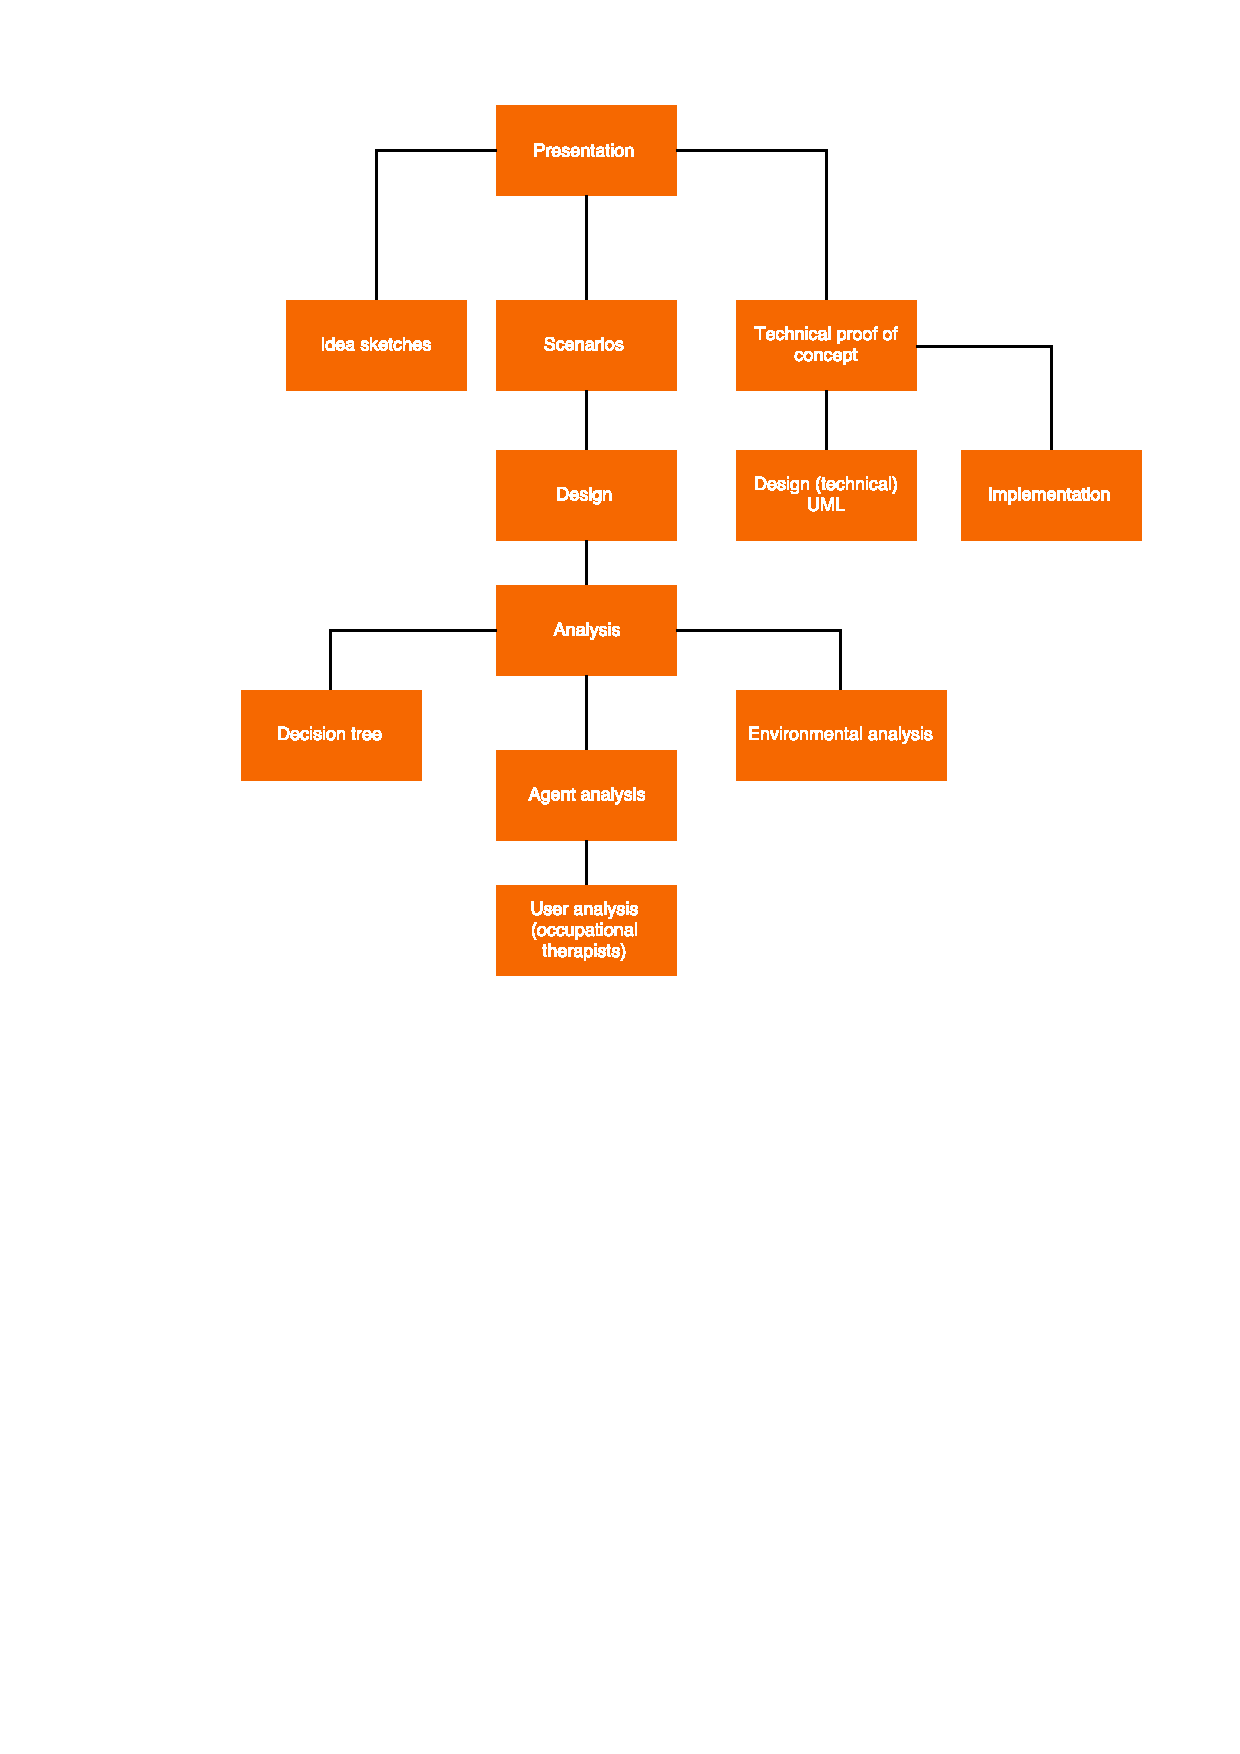
\includegraphics[width=\linewidth]{graphics/wbs.pdf} 
  }
  \caption*{}
\end{figure}




\end{document}
